Here we will show some results of finite differencing and of the stochastic methods. Figure~\ref{fig:FiniteDifferences} shows a simulation of a particle density for a certain amount of time. In this figure we see that the density tends to accumulate into the wells and that wherever the density has a sharp peak, it will interact with the environment thermally. The strength of these thermal interactions depends on $\kappa$ and for a non vanishing $D$ they tend to diffuse away into a smoother shape. If we allow these simulations to run for long enough, then eventually we will reach the predicted steady state.

\begin{figure}[tb]
	\centering
	\subfigure{%
		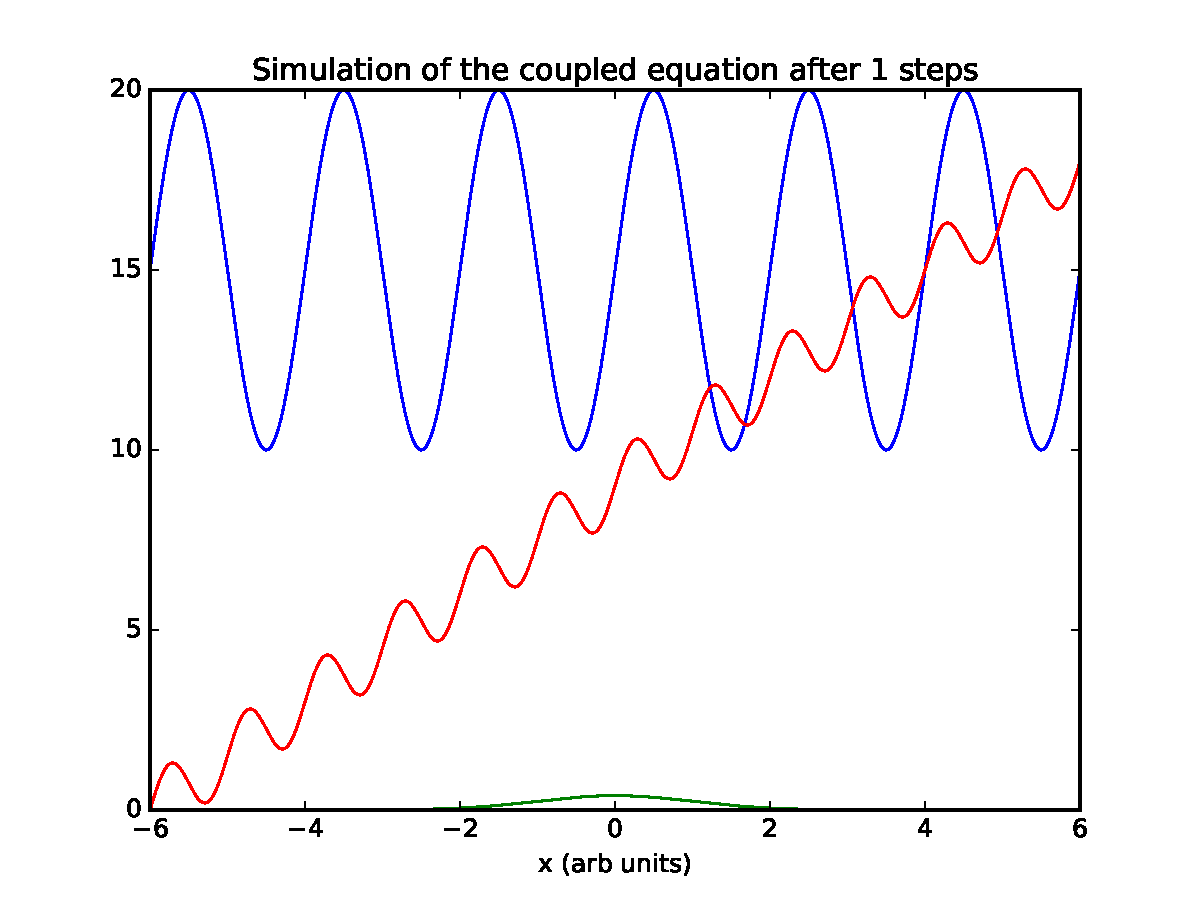
\includegraphics[width=0.45\columnwidth]{CoupledEquationFiniteDifferencesInitial}
	}
\quad
	\subfigure{
		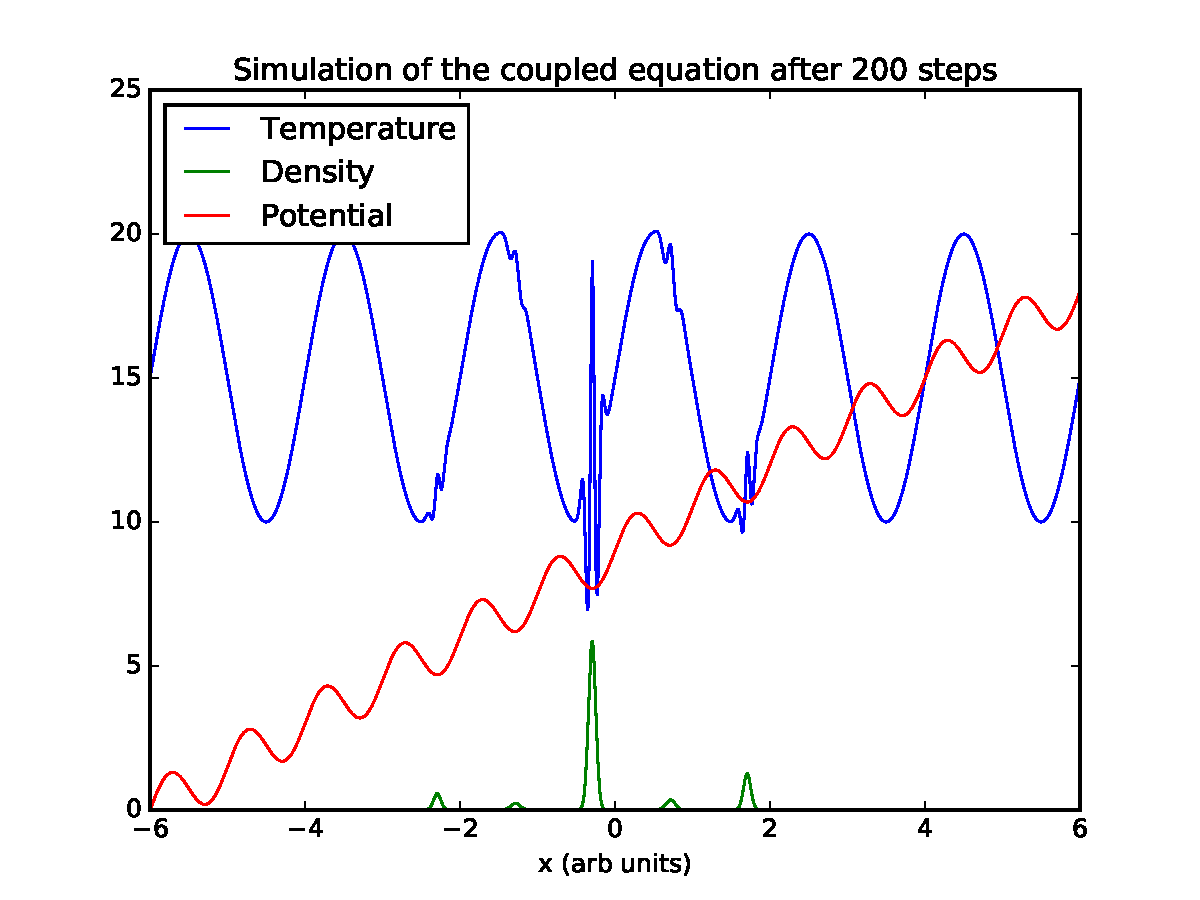
\includegraphics[width=0.45\columnwidth]{CoupledEquationFiniteDifferences}
	}
\caption{Finite differencing simulation of a distribution of particles, we see that the particles are locally interacting with the environment thermally.}
\label{fig:FiniteDifferences}
\end{figure}

\begin{figure}[tb]
	\centering
	\subfigure{%
		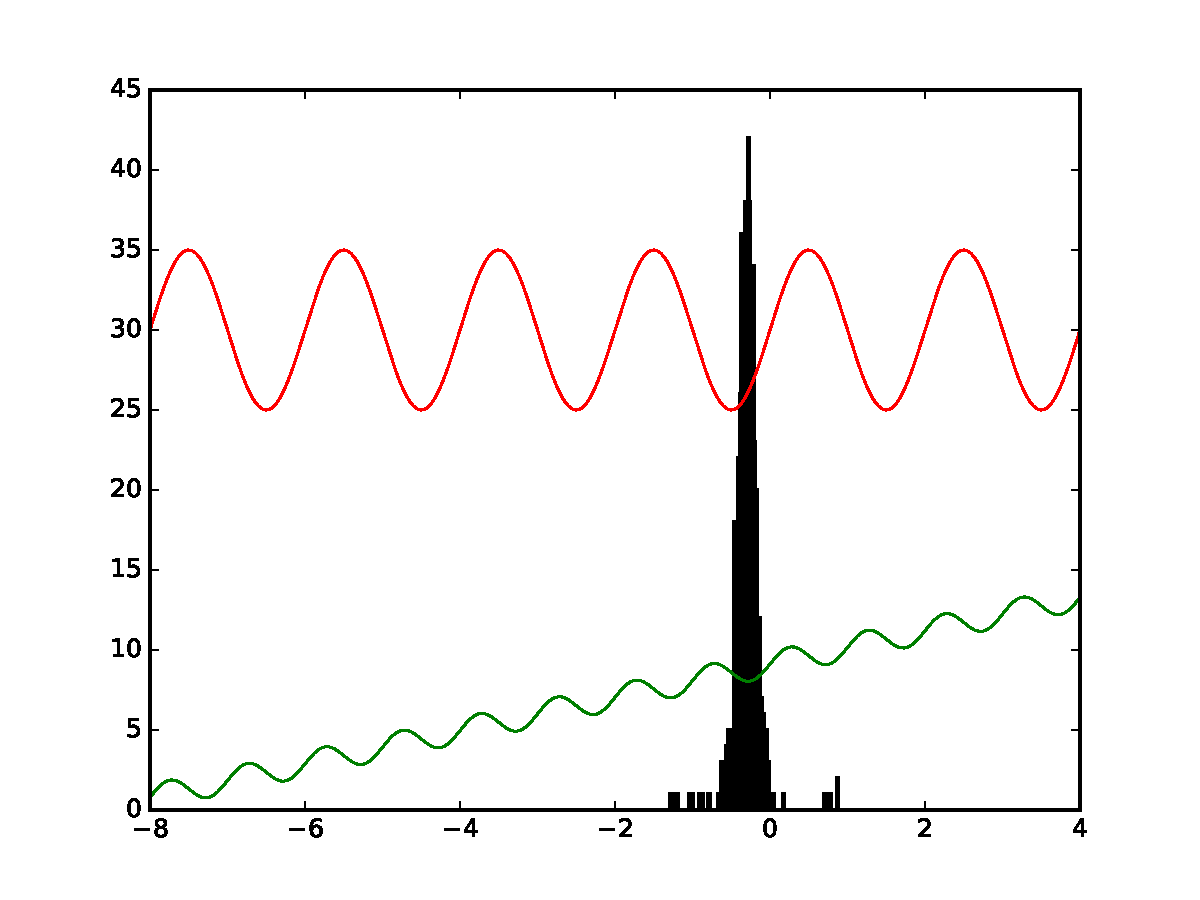
\includegraphics[width=0.45\columnwidth]{CoupledEquationStochasticInitial}
	}
\quad
	\subfigure{
		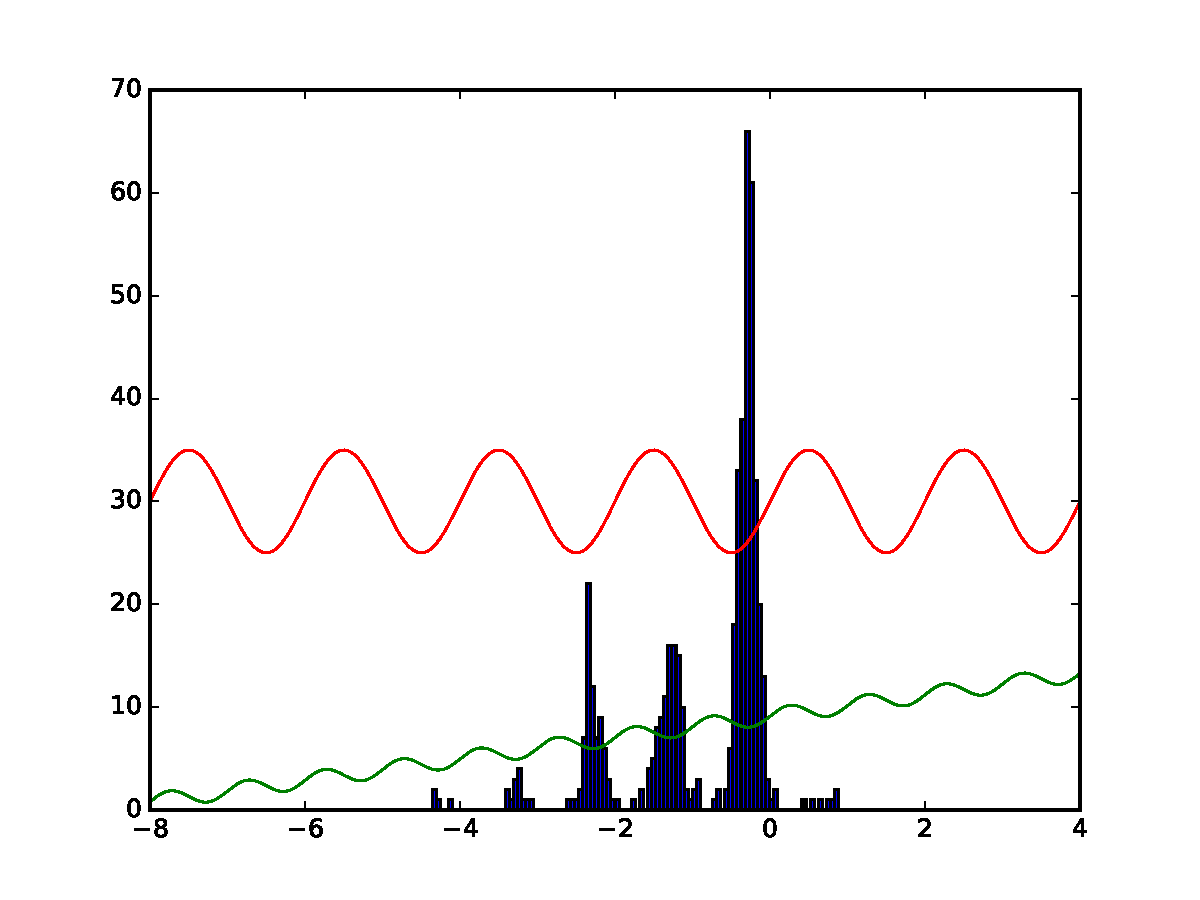
\includegraphics[width=0.45\columnwidth]{CoupledEquationStochastic}
	}
\caption{Stochastic simulation of a distribution of particles, In this simulation we have coupled the equations so that the diffusion of the particles is dependent on the temperature, however the temperature is not affected by the particles (i.e. in the case where $\kappa \to 0$).}
\label{fig:Stochastic}
\end{figure}

Meanwhile, figure \ref{fig:Stochastic} shows a similar situation that has been simulated stochastically. In this case, we  are able to deal with a temperature that is non constant in space, however we are not able to quantify the particles interaction with the environment. This means that $\kappa$ vanishes in our stochastic model. In the future, we aim to be able to deal with these thermal interactions by using the microscopic equations given by Streater \cite{Streater1997, Streater1997a}.
